\chapter{Morsesignalering}

\section{Inledning}

Många slags signaler har genom tiderna använts för att sända budskap.
Till en början användes akustiska och optiska signaler, det var rop, hornstötar,
rökpuffar, ljusblinkar, signalflaggor osv.
Under tidigt 1800-tal började man sända meddelanden med hjälp av elektriska
impulser genom ledningar.
År 1837 presenterade amerikanen Samuel~F.~B.~Morse en elektromagnetisk
skrivtelegraf.

Redan i början på 1840-talet hade han förbättrat apparaten och utvecklat ett
system, som i stort bibehållits in i våra dagar.
Flera andra personer har med tiden vidareutvecklat den teckenkod som Morse
först formulerade och kompletterat den med skiljetecken och ytterligare andra
tecken.
Koden kallas fortfarande MORSE-koden.
Kommunikationssättet kallas telegrafi och betyder fjärrskrift (av grekiskans
tele = fjärr och grafein = skriva).

Grundprincipen för telegrafi är densamma än i dag, men nu används mest
maskinella hjälpmedel, både vid sändning och mottagning.
Jämsides med morsekoden, som utformades för manuell signalering, har det
utvecklats signalkoder som är speciellt avsedda för signalering med t.ex.
teleprintrar, telefaxmaskiner och datorer.
Men trots den snabba tekniska utvecklingen överförs fortfarande meddelanden
manuellt med morsesignalering.
Metoden hävdar sig nämligen speciellt bra under svåra atmosfäriska och
trafikmässiga förhållanden samtidigt som den tekniska utrustningen kan vara
förhållandevis enkel.
Därför lever den 180-åriga morsesignaleringen vidare.

\section[Morsesignalering]{Morsesignalering inom amatörradion}

Med amatörradio har människor av många nationaliteter och med många olika yrken
och bakgrunder mycket goda kontaktmöjligheter.
Ett roligt sätt att ha kontakter över radio är då att morsesignalera.
Det är ett levande sätt att uttrycka sig.
Radioamatörer tar sig gärna en pratstund eller deltar i tävlingar på det sättet.
Det hindrar dock inte att många andra sändningsslag också kommer till
användning.

\section{Morsetecknen}

\begin{wrapfigure}{R}{0.5\textwidth}
  \fbox{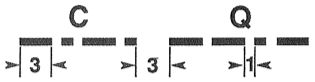
\includegraphics[width=0.5\textwidth]{images/cropped_pdfs/bild_morse_1.pdf}}
  \caption{Morsetecknens uppbyggnad}
  \label{fig:bild_morse_1}
\end{wrapfigure}

Bild \ref{fig:bild_morse_1} visar morsetecknens uppbyggnad.
Morsetecknen består av korta och långa teckendelar samt mellanrum.
Man utgår från den korta teckendelen vars längd sätts till en enhet.
En lång teckendel ska vara tre enheter lång, dvs. tre gånger längden av den
korta teckendelen.
Mellan teckendelarna inom tecknet ska mellanrummet vara en enhet långt.
Mellan hela tecknen inom ord eller teckengrupp ska mellanrummet vara
tre enheter långt och mellan hela ord eller teckengrupper sju enheter långt.
Morsetecknen finns standardiserade i ITU-R M.1677-1 \cite{M1677-1}.

\section{Planlagd övning}

Att delta i en organiserad kurs i den lokala radioklubben, FRO-avdelningen etc.
är bra, eftersom man då kan få en handledare och tillgång till övningsmaterial.
Inte minst viktigt är stödet av studiekamraterna.
Det går också att på egen hand lära sig att signalera, men det är ensamt och
därför kanske lite svårare.

För att lära morsesignalering måste man vara motiverad.
Det krävs nämligen tålamod och regelbunden träning.
Helst bör träningen ingå i den personliga dagliga rutinen, även om det bara
blir under några minuter.
Det går att hoppa över 1--2 dagar i veckan, men det bör då ingå i övningsplanen.
Att hoppa över ännu fler blir lätt en ovana.
Att träna lite då och då ger inget bra resultat.

\section[Inlärningsordning]{Ordning för teckeninlärning}

\begin{table}[h]
  \centering
   \begin{tabular}{|r|l|}
  	\hline
  	\textbf{Lektion} & \textbf{Nya tecken} \\ \hline
  	1 & L N E O = + (åtskillnad och slut) \\
  	2 & I X \\
  	3 & V T \\
  	4 & / ? $\surd$ (vänta) \\
  	5 & - x (repetition) \\
  	6 & A Z \\
  	7 & . \\
  	8 & H Ö \\
  	9 & 7 4 9 5 \\
  	10 & 8 1 \\
  	11 & 3 6 \\
  	12 & R D \\
  	13 & 2 0 \\
  	14 & F Y \\
  	15 & Ä B \\
  	16 & P S \\
  	17 & U Q \\
  	18 & W K \\
  	19 & Å M \\
  	20 & C G J \\
  	21 & $\sim$ (lystring) \\
  	22 & @ (avslutning) \\
  	23 & f (förstått) \\
  	24 & ........ (felslagning) \\
  	\hline
  \end{tabular}
  \caption{Inlärningsordning för morsetecknen}
  \label{fig:morse_ordning}
\end{table}

Inlärningsordningen enligt bild \ref{fig:morse_ordning} rekommenderas.
Man börjar med tecken som låter så olika som möjligt.
Detta för att undvika förväxling längre fram, när tecknen blir fler och
hastigheten högre.
Under inlärningen blandas nya tecken med de redan inlärda.
Följ kursens ordning och hoppa inte över något!
Öva utan avbrott så att hjärnan blir ordentligt ''programmerad''.
Det är lämpligt att lära in 2 till 4 nya tecken varje vecka.

\section{Inlärningstid}

Behövlig inlärningstid är mycket individuell.
För 40~tecken/minut, som motsvarade ett C-certifikat en gång i tiden, bör man
räkna med åtminstone 100 effektiva timmar för mottagning och 25~timmar för
sändning.

Att klara en taktökning till 60~tecken/minut och högre krav på säkerhet i både
mottagning och sändning, bör man räkna med ytterligare 25~timmar eller mer.

\section{Inlärningsmetodik}

Morsetelegrafi bör läras med beprövad metodik.
Bästa sättet är att man också skriver ner tecknen när man hör dem.
Metoden är s.k. ''nervbaning'' med målet att handen reflexartat skriver ett
visst tecken då en viss rytm hörs.
Att träna bara genom att höra tecknen är nästan verkningslöst.
Först när du lärt dej alla morsetecken grundligt genom mottagning är det dags
med sändningsträning.

\section{Mottagnings\-övningar}

Morsetecken är ju långa och korta teckendelar i form av ljud, ljus etc.
De kan även illustreras som långa och korta streck.
För att tecknen ska uppfattas som en melodi eller ljudföljd och för att man
inte ska frestas att räkna korta eller långa teckendelar är lämpligt att
morsetecknen lärs in i hög hastighet, men med förlängt mellanrum, s.k.
spärrad stil.
Det är själva ljudbilden som ska läras in.
I början kan det ändå vara svårt att låta bli att räkna teckendelar, men
efterhand uppfattar man trots allt tecknen som ljudbilder.

När man ska skriva mycket under en längre tid är sittställningen viktig.
För att inte bli trött ska man försöka inta en avslappnad sittställning och låta
hela underarmen vila mot bordet.
Använd papper med stora rutor och en bra kulspetspenna.
Skriv gärna på varannan rad så att det finns plats under att rätta texten.

För att spara tid bör man använda små handrörelser och inte lyfta pennan mer än
nödvändigt.
Studera skrivanvisningarna i slutet av detta kapitel.
Använd för tydlighetens skull textad stil, men tydlig skrivstil går också bra.
Lyssna på hela tecknet innan du skriver ner det.
Skriv lugnt.
Hoppa över tecken som du missar!
Försök inte att minnas tecken som du just missat.
Då kommer du nog att missa efterföljande tecken också.
Koncentrera dig i stället på tecknen som kommer.

Vissa morsetecken är så korta att det är svårt att hinna skriva ner dem.
För att spara tid måste vissa tecken skrivas i ett penndrag, t.ex. bokstäverna
M, N m. fl..
Bokstaven E som är det kortaste tecknet skriver man som en bakvänd trea
( \reflectbox{3} ).
Bokstaven U bör formas fyrkantig och bokstaven V spetsig, annars förväxlas de
lätt.
En nolla skrivs som Ø, med genomstrykning och en etta som 1.
En nolla utan streck kan lätt förväxlas med bokstaven O och en etta utan fot med
bokstaven I.

Var noga med handstilen från början och jobba hela tiden med att förbättra den.
En olämpligt inlärd handstil är mycket svår att arbeta bort och då får man
problem vid högre hastigheter.
Du ska ju själv kunna tyda din text i efterhand, men viktigast är att
provförrättaren också ska kunna läsa den.

Inlärningstexter är ofta uppdelade i grupper med 5 eller 4 tecken.
Dessa ska simulera ord.
Var noga med att du får tydliga ordmellanrum även på papperet.

\section[Eftersläpning]{Eftersläpning vid mottagning}

Tiden för vart och ett morsetecken varierar kraftigt.
För att få en lugnare nedskrivning bör man försöka hålla några tecken i minnet
och släpa efter med nedskrivningen.
Detta är nödvändigt i högre hastigheter och särskilt vid vissa
teckenkombinationer.

\emph{Läs inte!}
Det är frestande att försöka bilda ord av de bokstäver som man just skrivit ner.
Läsningen tar bort uppmärksamhet från mottagningen och det blir lätt
felgissningar.
Man tappar lätt den text som man just då tar emot.
Läs alltså inte och gissa inte på orden.
Täck över det skrivna med den lediga handen!

\section{Sändningsövningar}

Att telegrafera är att uttrycka sig.
De handsända morsetecknen ska vara tydliga, på samma sätt som att tal och
vanlig handskrift ska vara det.
Det är därför mycket viktigt att teckengivningen lärs in på rätt sätt.
Speciellt de första sändningsövningarna bör ske tillsammans med en kunnig
instruktör.
Om instruktör saknas -- följ då noga anvisningarna och var självkritisk!

\section[Övningshjälpmedel]{Hjälpmedel vid sändningsövning}

För sändningsövningarna behövs en dator med ljudfiler eller träningsprogram.
Vidare behövs en summer ansluten till en telegrafnyckel och en stereohörtelefon.
Eventuellt kan man ha en andra summer som nycklas av datorn och vars ljud matas
i en av hörlurarna.

Lär in sändning med en manuell telegrafnyckel och inte med en s.k. bug.
Vid provtagning blir man nämligen ofta nervös och då är det lätt att sända fel
med en bug.
Med en el-bug är risken stor för nya fel ''bara för att man råkat snudda vid fel
paddel'' därför kommer ett fel sällan ensamt.

\section[Ställning]{Arbetsställning vid sändning}

\begin{figure}
  \fbox{
    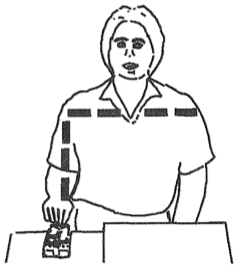
\includegraphics[width=0.5\textwidth]{images/cropped_pdfs/bild_morse_3.pdf}
    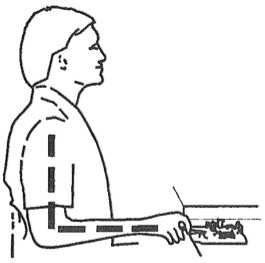
\includegraphics[width=0.5\textwidth]{images/cropped_pdfs/bild_morse_4.pdf}
  }
  \caption{Rätt sittställning sett framifrån och från sidan}
  \label{fig:bild_morse_3_4}
\end{figure}

Det är viktigt att ha rätt arbetsställning redan från början.
Vid hög sändningstakt och långa sändningspass blir man annars lätt trött och
får dålig teckengivning.
Över 60-takt börjar rätt arbetsställning att få stor betydelse.

Vid trötthet under sändning höjer man ofta axeln varvid armbågen åker ut.
Det blir då arbetsamt och man får ''bryta sig'' genom slutet på texten under
dålig teckengivning.

Bild \ref{fig:bild_morse_3_4} visar rätt sittställning.
Sitthöjden bör vara så att båda fötterna kan vila på golvet eller på en fotpall.
Telegrafnyckeln bör placeras så, att underarmen är vågrät när handen vilar på
nyckelknoppen.
Överarmen kan då hänga avslappnad rakt nedåt och över- och underarmen kan bilda
en rät vinkel.

Nyckeln bör vara fastsatt. Det är tyvärr vanligt, att nyckeln ställs löst på ett
olämpligt högt bord. Detta medför en olämplig och tröttande arbetsställning.

\section[Fattning]{Nyckelfattning och handrörelser}

\begin{wrapfigure}{R}{0.5\textwidth}
  \fbox{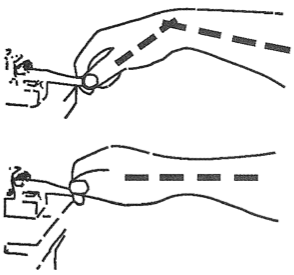
\includegraphics[width=0.5\textwidth]{images/cropped_pdfs/bild_morse_5.pdf}}
  \caption{Rätta handledsrörelser}
  \label{fig:bild_morse_5}
\end{wrapfigure}

Bild \ref{fig:bild_morse_5} visar nyckling med handledsrörelser.
Håll löst omkring nyckelknoppen med tummen och långfingret.
Pekfingrets undersida ska vila lätt ovanpå knoppen.
Använd alltid denna trefingerfattning.
Håll nyckelknoppen ganska långt in på fingrarna.
När man senare vill öka takten kan man flytta ut fattningen mot fingerspetsarna.

Morsetecknen skapas med rytmiska handledssvängningar uppåt/nedåt.
Håll inte hårt om knoppen -- men släpp den inte heller -- och spänn inte
handleden.
Handleden ska svänga mellan ett något upplyft och ett vågrätt läge.
I det vågräta läget når nyckeln sitt s.k. kontaktläge.
För att nästa tecken ska hinnas med i tid, får handleden inte svänga djupare än
till det vågräta läget.

\section{Styrd sändning}

Sändningsövningarna börjar med styrd sändning, men först sedan morsetecknen
lärts in grundligt genom lyssning.
Vid styrd sändning använder man stereohörlurar så att datorns eller
bandspelarens sändning hörs i den ena luren och den egna sändningen i den andra.
Den ton som nycklas hämtas från en generator som avger en konstant ton.

En textutskrift används som förlaga för den egna sändningen.
Det gäller att lyssna på morsetecknen från datorn eller bandet, samtidigt läsa
samma tecken från utskriften och själv sända dessa med nyckeln.
Ljudbilden från en egna sändningen ska då sammanfalla med den från förebilden.
På så sätt samövas hand- och armmusklerna, synen och hörseln för rätt
teckengivning.

I kurser på ljudband och data finns rytmiska ramsor för övning av styrd
sändning.
Börja med att öva ramsorna i nummerordning.
När man blir säkrare behöver man inte alltid träna alla ramsor.
Man känner själv vilka ramsor som man behöver öva mera.

Styrd sändning övas utan spärrning.
Teckenhastigheten och trafikhastigheten ska då vara lika.
Trafikhastigheten bör åtminstone vara 35 till 45 tecken/minut för
att teckenrytmen ska bli bra.
Träna mycket på siffror i den styrda sändningen.
Det ger färdighet vid övergångarna mellan korta och långa teckendelar i tecknen.
Även övergångarna mellan vissa morsetecken kan vara svåra.

\section{Fri sändning}

Först ska styrd sändning av ramsor och tecken klaras utan problem.
Börja först därefter med fri sändning utan ljudförebild.
Normalt ska sändning göras utan spärrning.

Försök komma ihåg teckenrytmen från den styrda sändningen.
Siffror och skiljetecken är svårast att sända.
Öva därför dessa tecken extra mycket.
Då blir också bokstäverna lättare att sända!

Sänd inte fortare än att handleden fortfarande arbetar mjukt vid kontaktläget,
men ändå distinkt.
Sändningen är ditt visitkort och därför krävs att den har kvalitet.

\begin{figure}
  \fbox{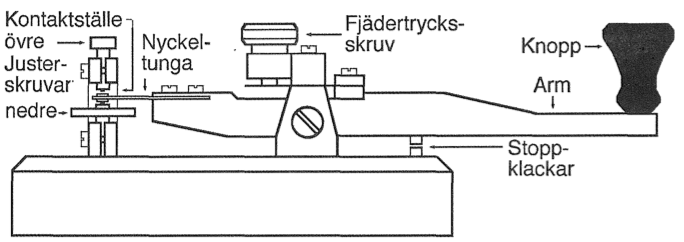
\includegraphics[width=\textwidth]{images/cropped_pdfs/bild_morse_6.pdf}}
  \caption{Telegrafnyckel}
  \label{fig:bild_morse_6}
\end{figure}

\section[Teckengivning]{Kontroll av teckengivningen}

Läsbarheten av den sändningsstil, som uppvisas vid certifikatsprovet, bedöms.
Ett i övrigt godkänt prov kan alltså bli underkänt p.g.a. dålig teckengivning.
Återkalla därför ett tveksamt utformat morsetecken och sänd om det, men var då
klar över att provtexten ökar med det antal tecken man sänder om.
Det innebär tidsförlust.

För kontroll av teckengivningen under sändningsprovet, och registreringen av
det, användes förr en teckenskrivare med pappersremsa.
Emellertid är en sådan skrivare numera ett svåråtkomligt hjälpmedel.

Det hjälpmedel, som i stället står till buds, är en ljudbandspelare, men tyvärr
har ju en sådan inte grafisk visning.
En telegraferingskunnig person bör därför anlitas för bedömning av
teckengivningen.

\section[Provtext]{Exempel på provtext}

.... ASCUNCION ÄR HUVUDSTAD I PARAGUAY, SOM LIGGER I SYDAMERIKA.
VID RADIOTELEFONERING UTGÖRES NÖDSIGNALEN AV ORDET MAYDAY OCH SKALL OM MÖJLIGT
UTSÄNDAS PÅ FREKVENSEN 2182 KHZ.
QRV? MEANS ARE YOU READY? THE RECEIVER CONTROL SETTINGS SHOULD BE ADJUSTED AS
INDICATED ON PAGE 3-4, DATED 7/10 1994. QRT + @

(summa 277 teckenvärden)

\section[Teckenvärden]{Beräkning av antalet teckenvärden}

Vid beräkning av antalet teckenvärden i en telegramtext ska bokstäver (utom Å)
räknas som ett (1) teckenvärde.
Siffror, skiljetecken, felsändningstecken samt bokstaven Å ska räknas som två
(2) teckenvärden.

I ovanstående exempel på provtext är fördelningen av teckenvärdena följande:

\begin{tabular}{lrcrcr}
Bokstäver          & 1 & $\cdot$ & 227 & = & 227 \\
Siffror            & 2 & $\cdot$ & 13  & = & 26  \\
Skiljetecken       & 2 & $\cdot$ & 12  & = & 24  \\
Summa teckenvärden &   &         &     & = & 277
\end{tabular}

Observera, att lystrings-, slut- och avslutningstecken samt felsända avsnitt med
respektive felsändningstecken också ska ingå i summan av teckenvärden.

Den därefter beräknade takten är den s.k. telegram- eller trafikhastigheten.

\section[Taktberäkning]{Beräkning av takten}

\textbf{Formel:}

$$\frac{\mathrm{summa\ teckenv"arde }\cdot 60}{\mathrm{tid} [\mathrm{sekunder}]}
= \mathrm{tecken/min}$$

\textbf{Exempel:}

Felfri sändning av ovanstående exempel på provtext med summa teckenvärde 277
tar exakt 4 minuter och 20 sekunder (260 sekunder).
Takten blir då:

$$\frac{277 \cdot 60}{260} = 63,9\ \mathrm{tecken/min}$$

\begin{figure}
  \fbox{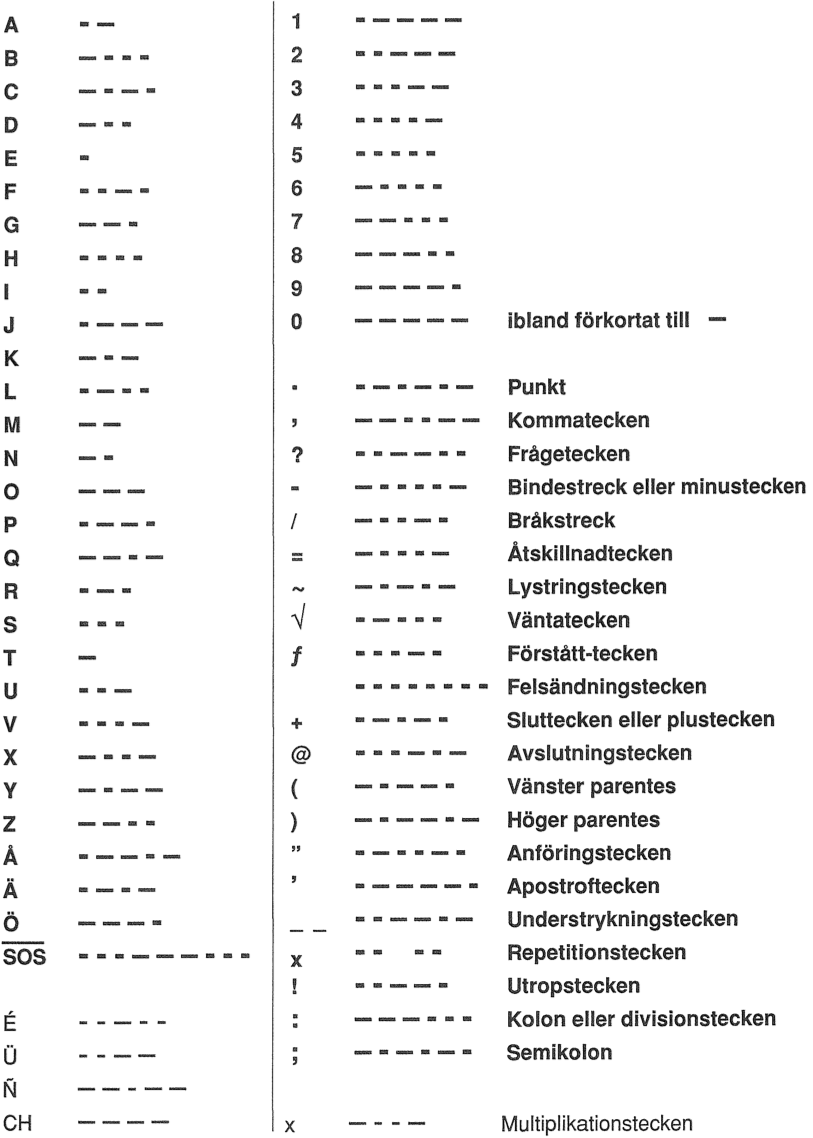
\includegraphics[width=\textwidth]{images/cropped_pdfs/bild_morse_7.pdf}}
  \caption{Morsealfabetet}
  \label{fig:bild_morse_7}
\end{figure}

\begin{figure}
  \fbox{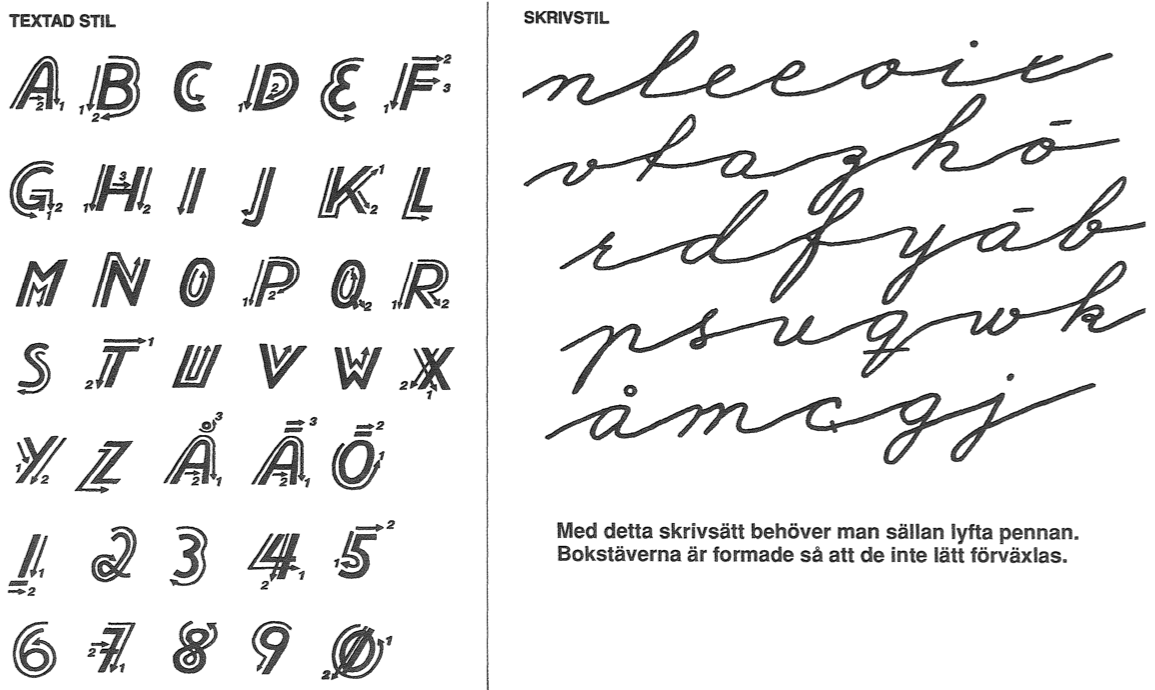
\includegraphics[width=\textwidth]{images/cropped_pdfs/bild_morse_8.pdf}}
  \caption{Handstilar}
  \label{fig:bild_morse_8}
\end{figure}
